\section{General Enhancements}
\label{sec:general-implementation}

In this section we describe the general architecture of the new prototype. 

\begin{figure*}[ht]
		\centering
        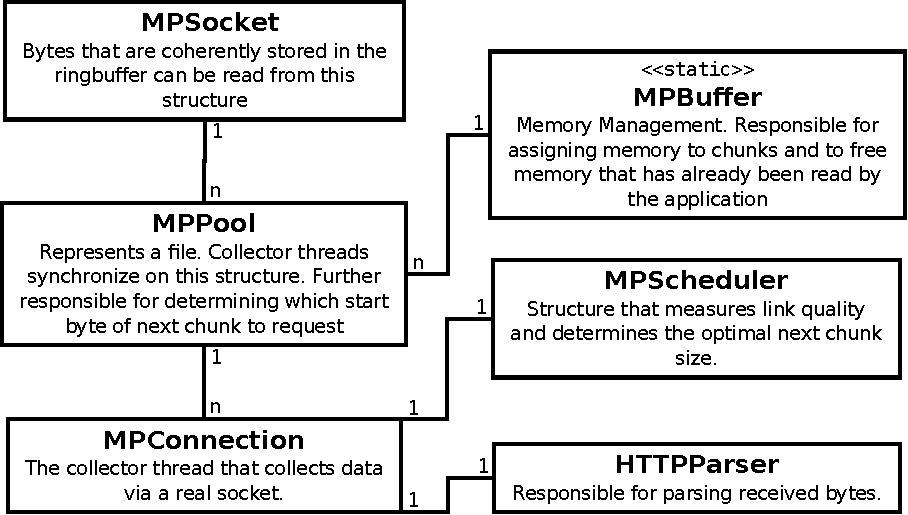
\includegraphics[width=0.7\linewidth]{Figures/implementation-uml.pdf}
        \caption{Illustration of \protonew~object relationships.}
		\label{fig:implementation-uml}
		\vspace*{-0.3cm}
\end{figure*}

In~\fref{fig:implementation-uml} the major objects and their relationships to each other are depicted. 
The \term{MPSocket} object acts as a multipath socket abstraction. 
It provides functions for reading coherently stored bytes via the \term{MPPool} from the \term{MPRingbuffer}. 
The \term{MPPool} object stores information about the running \term{Collector} threads, \ie \term{MPConnection} objects that are responsible for requesting and storing data in the \term{MPBuffer} over a path.
It also keeps track of chunks that still need to be requested and acts as a synchronization point for \term{MPConnection} threads. 
In order to successfully download chunks, each \term{MPConnection} object uses a \term{HTTPParser}, \ie a parser specifically designed and optimized for HTTP traffic, that recognizes different request and response header settings. 
Also, a \term{MPScheduler} object is used to determine the optimal next chunk size for a \term{MPConnection} object. 
Besides determining the optimal chunk size, the \term{MPScheduler} object also estimates the link quality of the path of the designated \term{MPConnection}. 
Through the \term{MPPool}, each \term{MPScheduler} object can make inquiries about the state and performance metrics of other \term{MPConnections}. 
Finally, one static \term{MPBuffer} object is used to manage memory requirements for the dynamic chunks. 

\subsection{New Threading Model}
\label{sec:threading-model}

The \protoold~prototype has exactly one thread that is responsible for sending requests and receiving and processing data from all the open TCP sockets. 
This thread is called \term{Collector} thread. 
Processing data means parsing and copying it into buffers, where the application can later read from. 
While parsing, copying and requesting data the \term{Collector} cannot drain data from any other TCP buffer. 
This behavior bears a potential bottleneck since the TCP buffers might be full before the \term{Collector} has time to drain them, which in return will reduce the TCP receiver window and will force the sender to reduce his sending rate. 
In order to avoid such a scenario it is of utmost importance to ensure that each receiving TCP buffer is drained as fast as possible. 

For that reason we propose a new threading model as illustrated in~\fref{fig:implementation-memory-management}, in which each TCP socket has its own dedicated \term{Collector} thread. 
Creating new threads is relatively expensive in terms of time and resources for the operating system, still this overhead is small compared to the possible gain from a higher parallelization to keep the connections busy and to avoid potential TCP buffer bottlenecks.
To appropriately handle higher parallelization a more sophisticated locking mechanism needs to be applied, which also results in higher overall implementation complexity and when implemented inefficiently might also lead to threads unnecessarily blocking each other which might then result in unnecessary processing overheads. 
To avoid this issue we use the locks only at the beginning of a chunk request. 
At the beginning of a request the thread needs to determine the next request range and allocate memory for the expected data. 
Further, in order to keep track of metrics such as the amount of requests sent, concurrent writes have to be avoided through locking. 
This means that during request preparation there is a chance of threads temporarily blocking each other, but since prior to a request there is no data that needs to be drained from the socket buffer no TCP buffer bottleneck can occur. 
The \term{Collectors} can receive and process data independently from each other, thus avoid an unnecessary blocking bottleneck during those phases. 

\subsection{Reducing System Calls}
\label{sec:system-calls} 

System calls such as memory copies (\eg memcpy) or memory allocations (\eg malloc, mmap) are expensive. 
Especially in case of very short download times, it is important to keep the processing overhead at the client side at a minimum. 
For that reason we change the data flow in \protonew~to reduce memory operations. 

\begin{figure*}[!htb]
		\begin{minipage}[t]{0.8\linewidth}
		\begin{center}
                \subfigure[Data flow in \protoold.]{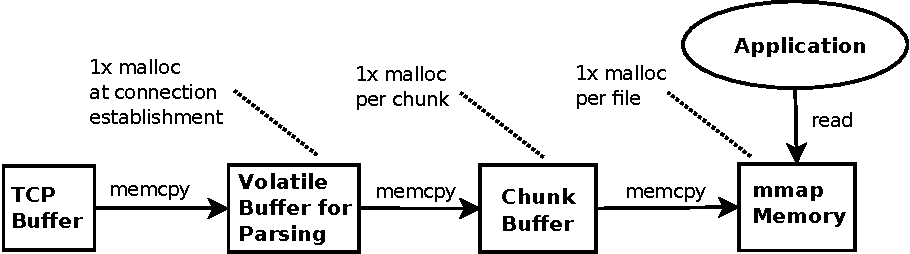
\includegraphics[width=\linewidth]{Figures/implementation-memcpy-old.pdf}}
				\subfigure[Data flow in \protonew.]{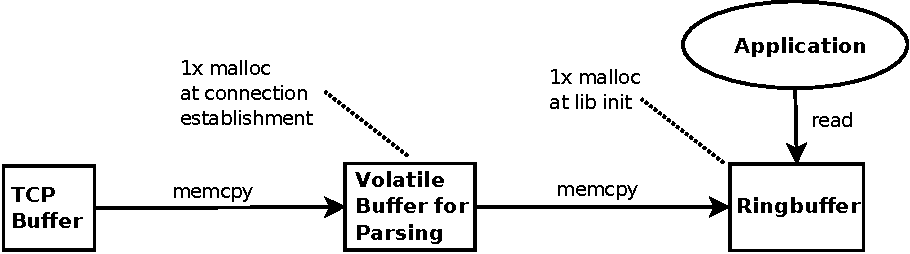
\includegraphics[width=\linewidth]{Figures/implementation-memcpy-new.pdf}}
        \end{center}
        \end{minipage}
		\caption{\label{fig:implementation-memory-flow} Data flow in \protoold~(a) and \protonew~(b).}
\vspace*{-0.3cm}
\end{figure*}

The data flow in \protoold~can be seen in~\fref{fig:implementation-memory-flow} (a). 
For each requested chunk, memory needs to be allocated. 
Note, that chunks might arrive out of order. 
Upon knowing the file size of a web object, \protoold's \term{Collector} allocates the necessary memory for the whole file in assembled state with mmap. 
The \term{Collector} drains data from the TCP buffer into a volatile buffer in which the data is parsed. 
After parsing, the data is copied to its dedicated chunk memory. 
Once two coherent chunks are detected, their data is copied to the mmap allocated file buffer. 
As a result, $3$ memory copies and $1$ memory allocation per chunk plus $1$ memory allocation per file and per established connection are necessary. 

As can be seen in~\fref{fig:implementation-memory-flow} (b), \protonew~does not use a chunk buffer any longer. 
The logical chunk structures reserve memory directly from the ringbuffer instead of allocating their own memory, thus after parsing inside the volatile buffer, data is directly copied to the ringbuffer itself. 
Note, that like in \protoold~chunks can still arrive out-of-order. 
The \term{MPSocket} and \term{MPPool} objects as shown in~\fref{fig:implementation-uml}, are responsible for delivering the data coherently to the application. 
Further, \protonew~only allocates ringbuffer memory once at library initialization time. 
This means, that in total $2$ memory copies per chunk, $1$ memory allocation per established connection and $1$ initial memory allocation at library start time are necessary, thus greatly reducing the amount of system call compared to \protoold. 

Finally, \protonew~also reuses already allocated objects, thus reducing the amount of expensive memory allocations for small objects, \ie \term{MPConnection} and \term{MPPool} objects are all reusable now. 

\subsection{Memory Management}
\label{sec:memory-management}

\protonew~comes with a more advanced memory management than \protoold. 
In \protoold~each chunk needed a memory allocation. 

\begin{figure*}[!htb]
        \begin{minipage}[t]{0.8\linewidth}
		\begin{center}
                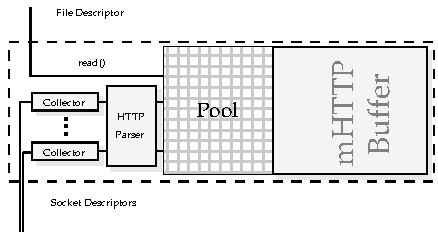
\includegraphics[width=\linewidth]{Figures/design-buffer.pdf}
				\caption{\label{fig:implementation-memory-management}multiHTTP design: I) \mhttp~buffer stores out-of-order received data II) HTTP parser examines and modifies HTTP headers III) collectors gather data from individual TCP connection buffers.}
        \end{center}
        \end{minipage}
  \vspace*{-0.3cm}
\end{figure*}

In contrast, upon initializing the \protonew~library, a simple ringbuffer with a fixed size is created in which data can be stored. 
The application reads directly from the ringbuffer via the \term{MPPool} as shown in~\fref{fig:implementation-memory-management}. 
Instead of allocating new memory each time a chunk of a dynamic size is requested, memory space from the ringbuffer is used, thus saving expensive system calls. 
Moreover, using a ringbuffer allows us to easily keep track of coherently stored bytes. 
Note, that the only requirement for data to be delivered to the application is coherency, meaning that even if a chunk is not completely downloaded, as long as it is coherent, even parts of it can already be read by the application.
This eases the correct delivery of coherent data to the application. 

In this proof-of-concept stage we use wget~\cite{URL-WGET} to download files. 
Since wget does not request files in parallel, but sequentially, a ringbuffer is the easiest, yet efficient choice. 
Note, that in order to work with applications which request files in parallel (such as web browsers like Firefox) another memory management strategy needs to be developed, but that is subject to future \mhttp~implementations. 



